\chapter{Penetration testing} \label{ch:pentesting}
This chapter details all penetration tests that were performed on the system. These were derived from the threat model created in chapter \ref{ch:threat-model}. All penetration tests are described in the format outlined below. If an aspect of the test was considered simple then one or more parts have been omitted.
\begin{itemize}
    \item \textit{Introduction}. Describes the attack vector that this penetration test will explore.
    \item \textit{Background}. Details the required background knowledge to perform and evaluate this penetration test, if any.
    \item \textit{Method}. Describes in detail how the test was performed, e.g in what environment, with what tools, what commands were used, etc.
    \item \textit{Results}. Describes the findings of the penetration test.
    \item \textit{Discussion}. This section contains a discussion about the reliability, validity, and generalizability of the results.
\end{itemize}

\section{Lab Environment} \label{ch:pentesting:lab-setup}
This section describes the lab environment and physical setup used when performing the pentests described below.

For the pentests involving the RF communication between the devices of the system specific hardware is required. Specifically, a Software Defined Radio (SDR) is required to be able to receive and transmit RF signals. The SDR used in this report is the HackRF One\footnotelink{https://greatscottgadgets.com/hackrf/one/}{2021-05-17} from Great Scott Gadgets\footnotelink{https://greatscottgadgets.com}{2021-05-17}. This is a popular and relatively cheap SDR, costing around 350 USD. Additionally, an ANT 500 antenna was used since the HackRF One does not come with an antenna. As for the physical setup, the RF transmitting devices of the system were placed relatively close to the SDR, within \texttt{10-20 cm}. This was done to increase the quality of the captures. By placing them close clean signals could be captured without increasing the gain parameters of the SDR. Figure \ref{fig:rf-lab-setup} shows a picture of the physical lab environment.
\begin{figure}[!ht]
    \centering
    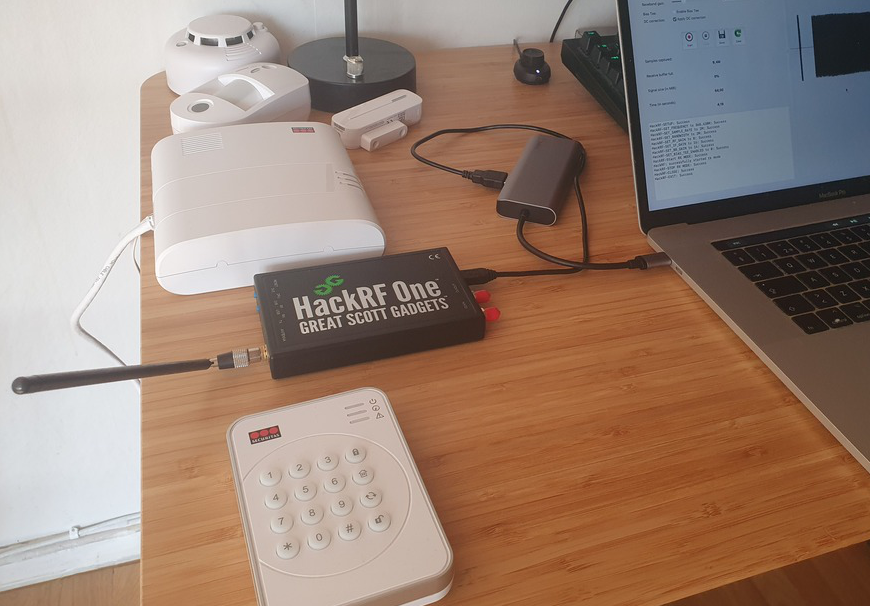
\includegraphics[width=0.9\textwidth]{images/6-pentesting/lab-setup.png}
    \caption{The lab setup used to capture and replay RF signals.}
    \label{fig:rf-lab-setup}
\end{figure}

\section{Task 1: Climax Technology's Vesta platform} \label{ch:pentesting:vesta}
Climax Technology, the manufacturer of the hardware used in this system, does not seem to be a consumer-facing business. Nonetheless, they have their own software platform to control their system, called \textit{Vesta}. In the SecuritasHome system, this platform and its components are essentially replaced by \textit{Alarm.com}. The Vesta platform features a mobile application\footnotelink{https://play.google.com/store/apps/details?id=com.climax.vestasmarthome.eu}{2021-04-20} to control the system, as well as a web portal\footnotelink{https://eu.vestasmarthome.com/Vesta/}{2021-04-20}. A potential security vulnerability is if this Vesta platform is still active and usable to control this system.

\subsection{Background}
As stated above, Climax Technology have their own platform, branded as Vesta, to control the system. A common vulnerability in IoT devices is not covering up vulnerabilities arising higher up in the supply chain (\todo source). In this system, there is a possibility that \textit{Alarm.com} has not properly deactivated the access and functionality of the Vesta platform. The idea is for the Alarm.com platform to replace it entirely.

In the app \textit{Vesta Home 5 EU}, see figure \ref{fig:vesta-home-app}, one can perform essentially all actions that the Alarm.com mobile application provides (see section \ref{ch:system:software}). On the landing page, you are greeted with simple a login page (where your Alarm.com credentials don't work). However, it also includes a button labeled \textit{First Time Registration} (see figure \ref{fig:vesta-landing-page}), where one can register a new account connected to a new system. To register a new system one only needs to enter its MAC address, see \ref{fig:vesta-registration-page}, which is available without authorization from the local admin page (see \ref{ch:system:software}). Potentially, one could then register the system in the Vesta platform to gain authorization to control the system, thus bypassing the security completely.
\begin{figure}[!ht]
    \centering
    \begin{subfigure}[t]{0.4\textwidth}
        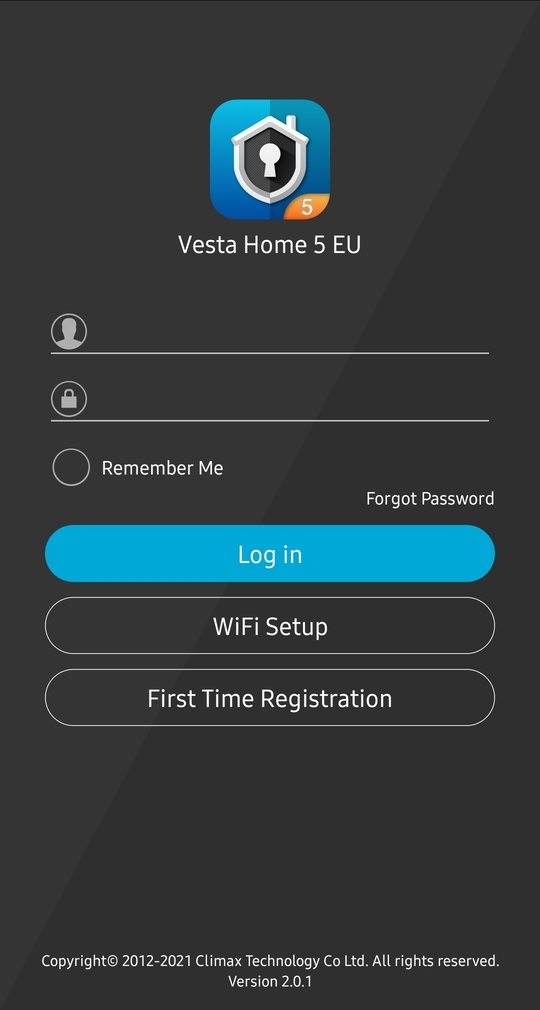
\includegraphics[height=3.8in]{images/6-pentesting/vesta-home-landing-page.jpg}
        \caption{The landing page}
        \label{fig:vesta-landing-page}
    \end{subfigure}%
    ~
    \begin{subfigure}[t]{0.4\textwidth}
        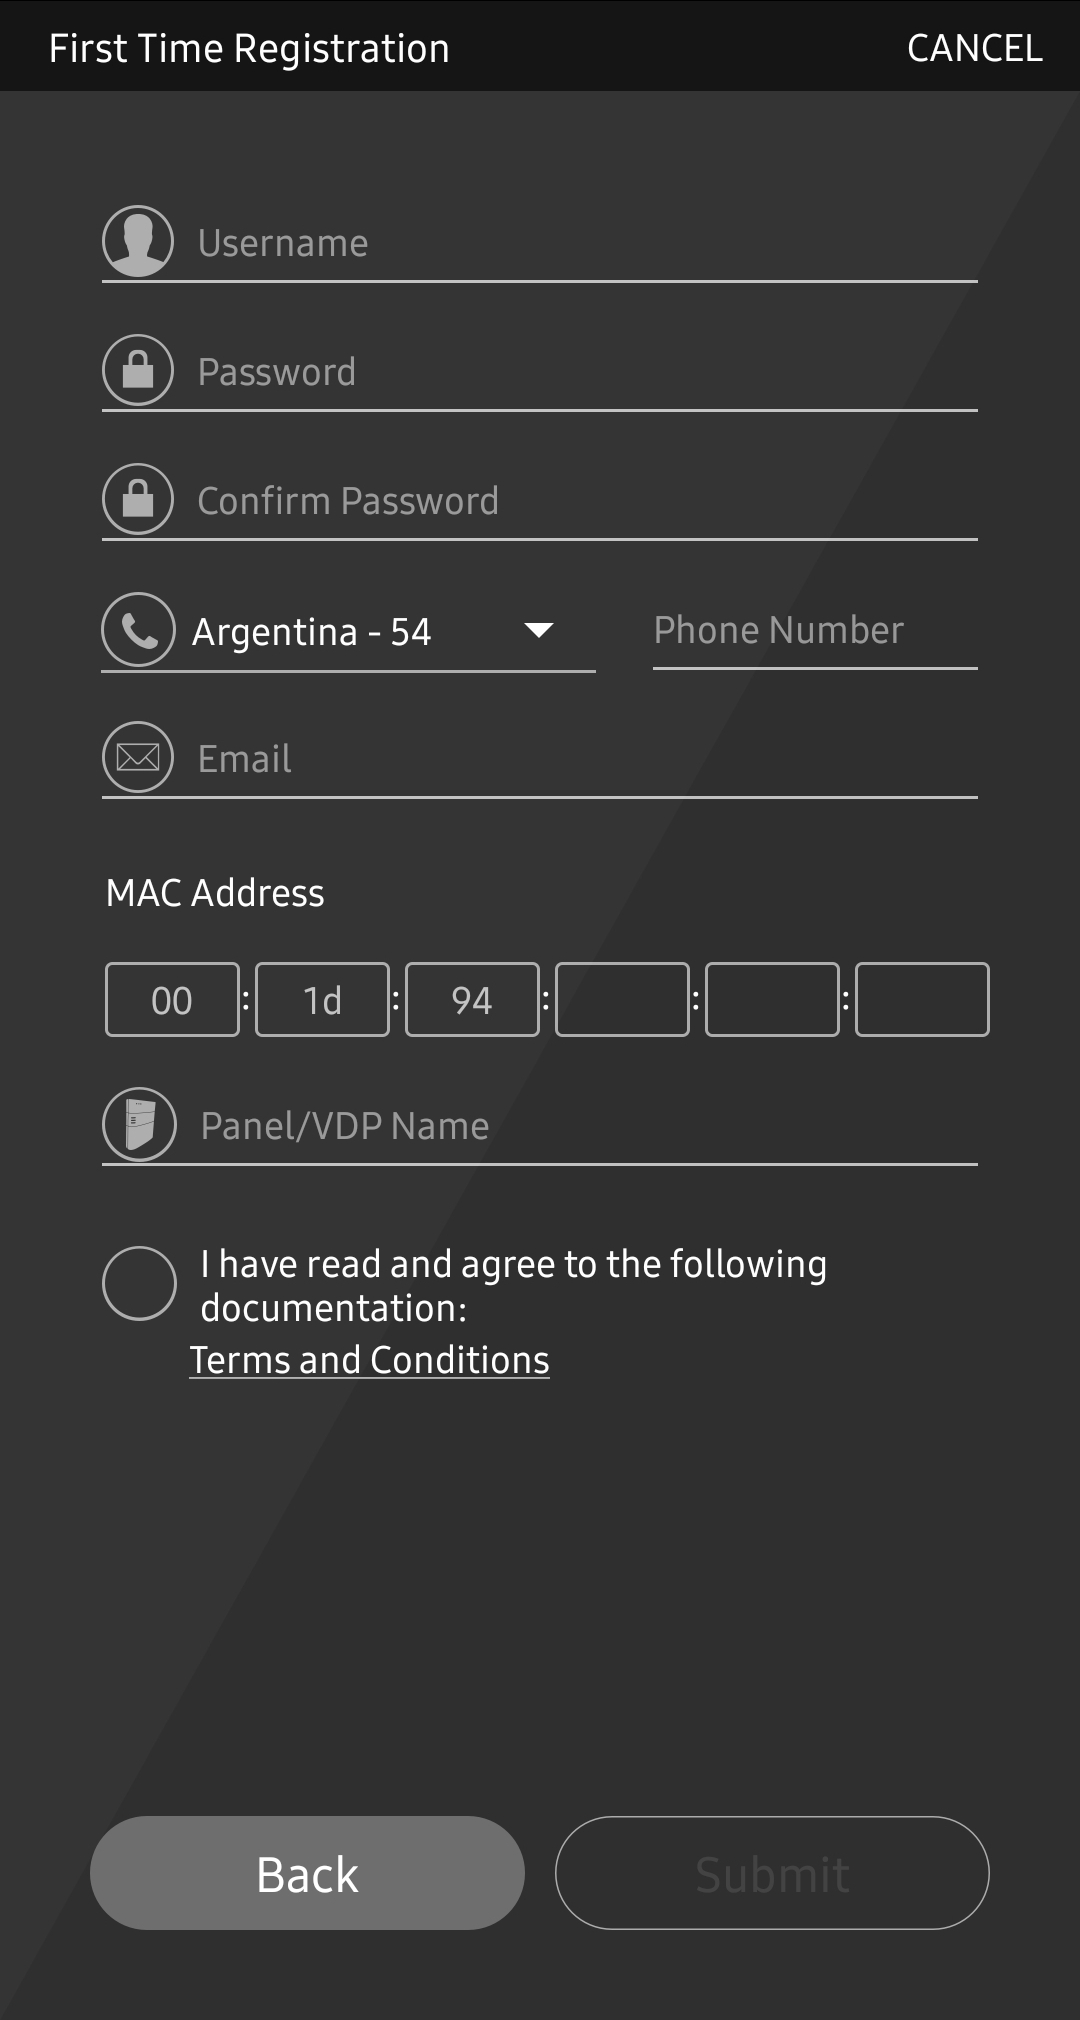
\includegraphics[height=3.8in]{images/6-pentesting/vesta-home-registration.jpg}
        \caption{The "First Time Registration" page}
        \label{fig:vesta-registration-page}
    \end{subfigure}
    \caption{The Vesta Home 5 EU mobile application.}
    \label{fig:vesta-home-app}
\end{figure}
In the Vesta web application, there is a very similar form, allowing you to register a new device using the MAC address, see figure \ref{fig:vesta-web-registration}.
\begin{figure}[!ht]
    \centering
    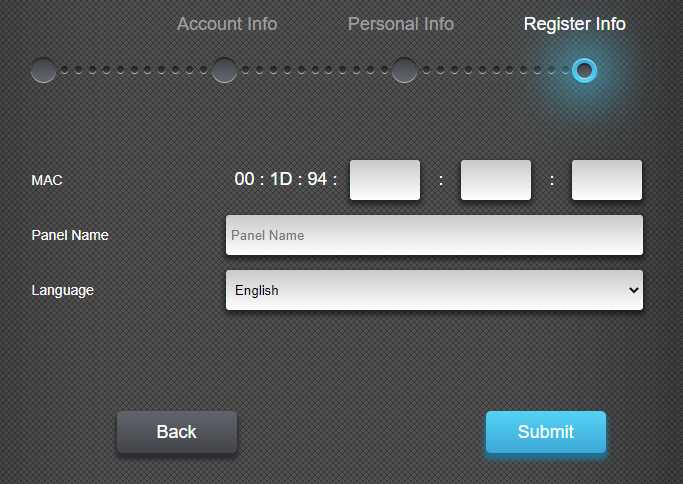
\includegraphics[width=0.9\textwidth]{images/6-pentesting/vesta-web-registration.png}
    \caption{The Vesta web application registration.}
    \label{fig:vesta-web-registration}
\end{figure}

\subsection{Method}
The mobile application is free to download. To be able to confidently monitor the network traffic, the mobile application was installed on an android emulator for PC, and Wireshark was run on the host machine.

Both applications use HTTPS, meaning the requests are encrypted. An attempt was made to perform a \gls{MITM} attack on the mobile application to view the HTTPS traffic, using \textit{mitmproxy}\footnotelink{https://mitmproxy.org/}{2021-04-21} and the built-in proxy settings of the android emulator. However, this made the application yield an error message saying it could not reach the server. Presumably, the application uses certification pinning to protect against this type of attack. This was not explored further since the traffic can easily be viewed in the web application, using the Chrome network tab (see figure \ref{fig:vesta-web-registration-failed}), and most likely both applications access the same API.

\subsection{Results}
The penetration test was unsuccessful. Both the mobile application and the web application yielded identical results. A simple error message is shown, saying the \textit{MAC/IMEI} is incorrect, see figures \ref{fig:vesta-home-registration-failed} and \ref{fig:vesta-web-registration-failed}. In the Chrome network tab, we can see when trying to register the system through the web application that the API responds with the message "no data found!".
\begin{figure}[!ht]
    \centering
    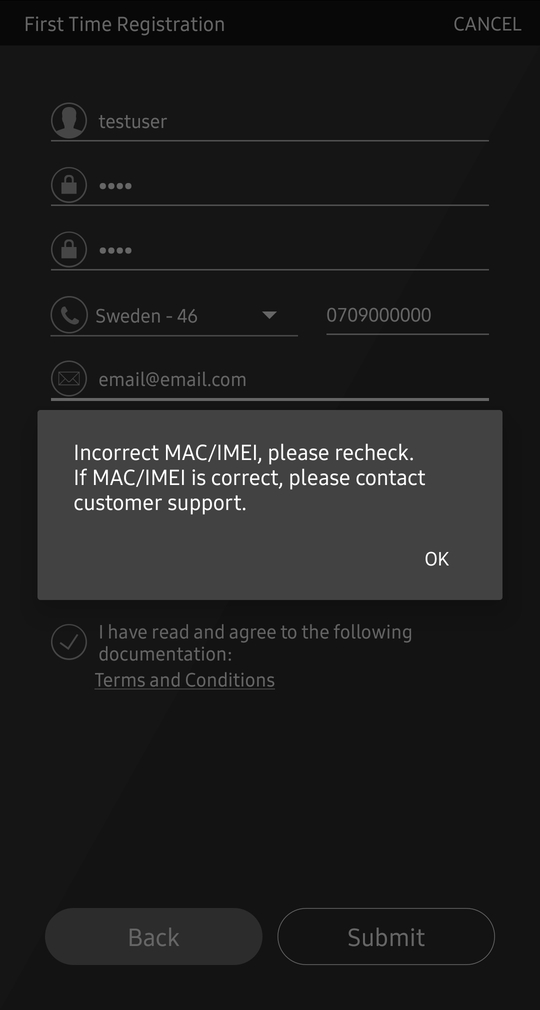
\includegraphics[width=0.4\textwidth]{images/6-pentesting/vesta-home-registration-failed.jpg}
    \caption{The results of trying to register in the Vesta mobile app.}
    \label{fig:vesta-home-registration-failed}
\end{figure}
\begin{figure}[!ht]
    \centering
    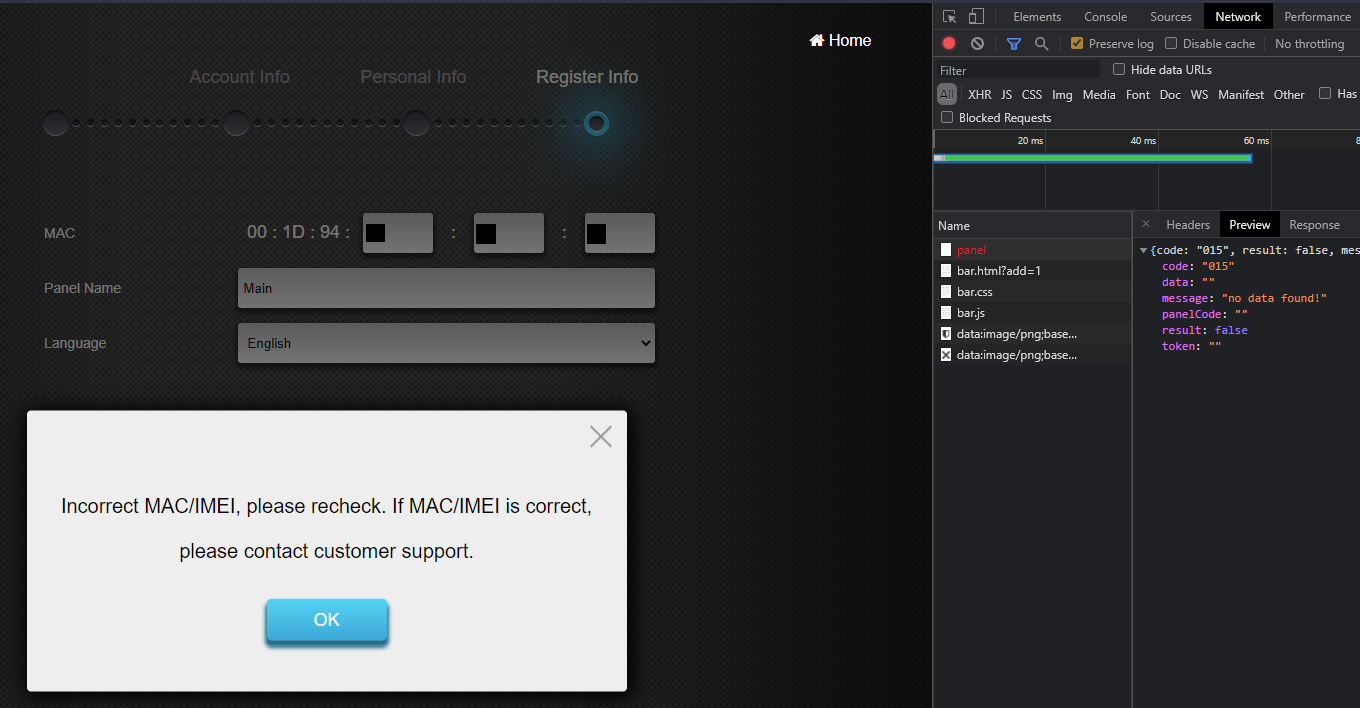
\includegraphics[width=0.9\textwidth]{images/6-pentesting/vesta-web-registration-failed.png}
    \caption{The results of trying to register in the Vesta web app.}
    \label{fig:vesta-web-registration-failed}
\end{figure}

\subsection{Discussion}
Trying to register the hardware to the Vesta platform was unsuccessful. The given MAC address was not accepted. Presumably, Climax Technology has a database of the MAC addresses of all sold systems under the Vesta platform. While the MAC address of the system in this thesis is registered under Climax Technology, it does not seem to be registered by the Vesta platform. Another possibility is that the MAC address and IMEI number pair is not registered because \textit{Alarm.com} has used their own SIM cards and thus a different IMEI number. This is indicated by the error messages shown. Which of these scenarios is the correct one, we cannot know. Either way, we can see that the API responds with a negative result, saying that no data could be found. Therefore, this type of supply chain error seems to have been identified and correctly protected against.

\section{Task 2: Online Password Attack} \label{ch:pentesting:password}
An online password attack refers to probing an active login, as opposed to an offline attack where you for example might try to crack a hash of a leaked database. This attack involves using some type of approach to test many passwords of a login form to try and find valid credentials. The local web admin page (see section \ref{ch:system}) has a login page that could potentially be brute-forced.

\subsubsection{Background}
A password attack, or password cracking, refers to cyber-attacks where the attacker tries to figure out valid credentials, to gain authorized access to a system. These can be categorized into two groups: offline and online password attacks. The former refers to attacks requiring no communication with the system in order to test a valid password. An example could be listening in on network traffic and seeing a password hash. One could then perform an offline password attack by trying to figure out which password produced that hash, and thus login to the system. In an online attack, the system under attack is in continuous communication with the attacker. This could be, for example, writing a script to try many different passwords on a login page of a web page. Online password attacks are generally harder to successfully perform. They are often much slower, as the communication with the system incurs a major overhead, and also poses the potential risk of getting caught in the middle of it if the administrator of the system notices the malicious traffic. Servers also often implement rate-limiting against IP addresses to combat these types of attacks and DOS attacks.

For both online and offline password attacks, there are several techniques one can use to try and guess the correct password. The simplest one is a \textit{brute-force attack}, where the attacker simply tries all possible passwords up to some length. Given $c$ possible characters in the password and a password length of $l$, there are $c^l$ possible passwords to try. This has exponential complexity in the length of the password, and will thus scale very poorly with longer passwords. Another technique is called a \textit{dictionary attack}, where the attacker uses a large list of known common passwords. Often these lists are created from actual passwords from leaked databases. For offline attacks like hash-cracking, there are additional techniques like \textit{rainbow tables}.

In the case of the system in this thesis, we have no opportunity for an offline password attack, as no information about the password such as a hash is leaked as far as the author is aware. The local admin web page does, however, feature a login page. This page uses \textit{HTTP Basic authentication} to log in to the main panel (see figure \ref{fig:local-login-page}). If this login system has not implemented any form of rate-limiting then guessing the right password might be possible, given enough time and resources.

\subsubsection{Method}
We know from sources like the one covered in section \ref{ch:related-work:lupus} that \textit{admin} is most likely a valid user name. This is further indicated by the official user manual from Climax Technology\footnotelink{https://fccid.io/GX9HSGWF1919/Users-Manual/Users-Manual-4873123}{2021-04-22}, which includes default login credentials with the admin user name (the credentials do not work on this system). As stated, the login form (see figure \ref{fig:local-login-page}) uses \textit{HTTP Basic authentication} to authenticate the user. A dictionary attack was performed against this login page. The well-known password list \textit{rockyou.txt}\footnotelink{https://github.com/danielmiessler/SecLists/blob/master/Passwords/Leaked-Databases/rockyou-20.txt}{2021-04-25} was used as the dictionary. A useful program to perform online password attacks is called \textit{Hydra}\footnotelink{https://github.com/vanhauser-thc/thc-hydra}{2021-04-21}, which is a command-line tool. Using the following command, Hydra was used to perform the attack:
\begin{lstlisting}[frame=tb]
    hydra -l admin       \
          -P rockyou.txt \
          192.160.1.90   \
          http-get       \
          "/action/login:F=Access Denied"
\end{lstlisting}

\subsubsection{Results}
The test was mostly unsuccessful. A password attack against the system was successfully executed. However, Hydra only manages to perform around 23 requests per minute against the main panel, see figure \ref{fig:hydra-password-attack}. This is too slow to be able to guess enough passwords to have a meaningful probability at a correct guess.
\begin{figure}[!ht]
    \centering
    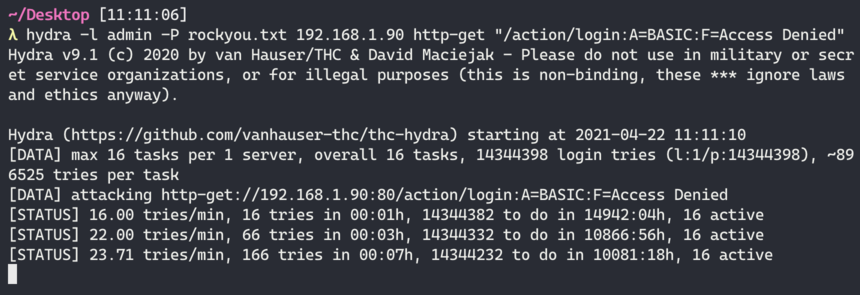
\includegraphics[width=\textwidth]{images/6-pentesting/hydra-results.png}
    \caption{The results of running a password attack.}
    \label{fig:hydra-password-attack}
\end{figure}

\subsubsection{Discussion}
The Hydra tool was only able to do around 23 requests per minute. Hydra is known to be very fast, so that is not the issue. One explanation for why this was so slow could be that the server rate-limits users. This is a common technique to protect against password attacks, if enough failed login attempts occur from a single IP the server would temporarily block or throttle it. However, there are signs indicating that this is not the case. For example, accessing the main web page slows down tremendously while performing the attack. Initially, it had around a \textit{16ms} response time, which increased to over \textit{17 seconds} during the attack. This was even confirmed on another computer, indicating that the main panel has not implemented any form rate-limiting per IP address. Presumably, the system is instead simply resource-bound and cannot serve requests at a faster rate. Given the hardware of the system, this is not unlikely. The CPU is most likely not that powerful, as is often the case in \gls{IOT} systems.

Due to the main panel not being able to serve more than 23 requests per minute, this type of attack is not feasible. For example, running a brute force attack, testing just all possible eight-character passwords, would take well over a hundred thousand years. A well-crafted dictionary attack could perhaps be effective, even at these slow speeds. However, there is some indication that the password might be just a random string of characters, given that the default password cited in the user manual is \texttt{cX+HsA*7F1}. If that is the case then a brute force technique is the only possibility. For these reasons, the attack was deemed unfeasible and not pursued further.

\section{Task 3: Replay attack on the RF communication} \label{ch:pentesting:replay}
This section details a penetration test against the RF communication between the hardware devices of the system. The specific attack vector explored in this section is a replay attack.

\subsection{Background}
A replay attack is an attack in network communication. The attacker listens in on the network traffic and simply retransmits the whole packets or information discovered in the packets to perform authenticated requests against a system they would otherwise not be able to. This type of vulnerability can have devastating consequences since even if several security measures have been taken, such as encrypting the data, the system can still be vulnerable to replay attacks. The attacker needs no knowledge of how the message is structured or what it contains.

Remote Keyless Entry (RKE) systems are notorious for being vulnerable to replay attacks. A famous example is RKE systems used in car keys, used to unlock a car with from a distance a press of a button. When these first arrived on the market the security was extremely lacking and researchers in 2016 found that many cars on the market have used these insecure systems for over 20 years \cite{car-rke-systems}. Often one-way communication from the key to the car over RF signals is used with no protection at all against replay attacks. Simply capturing the RF signal and replaying it would unlock the car. A simple and well tested protection against replay attacks is sending time-stamps along with your message. If the time stamp is older than some threshold when the receiver would reject the message \cite{rke-replay}. This can, however, sometimes be difficult to implement in embedded systems since it requires both parties to agree on the time. For devices with an internet connection this is easy thanks to the Network Time Protocol (NTP)\footnotelink{https://tools.ietf.org/html/rfc5905}{2021-05-03}. However most low-powered simple IoT devices, such as a car key, does not have internet-connectivity. A solution many modern systems used is a rolling code scheme. Both systems keep an initially synchronized internal code $C$. When the transmitter sends a signal it includes this number and increments it internally. The receiver stores the last such number it received and checks that the number in the new signal is within some interval $[C+1, C+K]$, for some constant $K$. If it is not then the number is rejected. In practice one might use this number to encrypt the message, or use a pseudo random number generator sequence instead of an integer $C$. This technique protects against replay attacks, however it is still vulnerable against what is called a \textit{rolljam attack} \cite{kamkar2015drive}. By jamming the signal and at the same time recording it the attacker now has a signal they can replay to have one time access to unlock the system. Most modern cars are still susceptible to this type of attack.

\subsection{Method}
To receive and transmit radio signals specific hardware is required. The hardware used in this project was an HackRF One\footnotelink{https://greatscottgadgets.com/hackrf/one/}{2021-05-12}, which is a popular and relatively cheap \gls{SDR} (around 300 USD). It plugs in to a computer using a USB cabel, which can then control the SDR. While low level protocols exist to control the HackRF One, one usually use more higher level tools to interact with it. The method of this pentest builds on the open source tool \textit{Universal Radio Hacker} (URH), which was created by researchers at Hochschule Stralsund – University of Applied Sciences in Germany \cite{urh}. Figure \ref{fig:rf-lab-setup} shows a picture of the lab setup used to perform this test.
\begin{figure}[!ht]
    \centering
    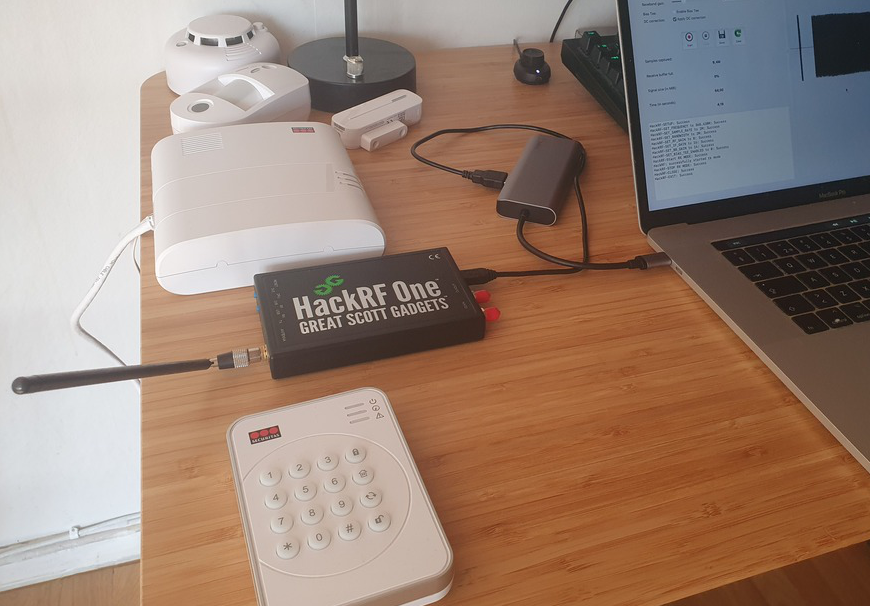
\includegraphics[width=0.9\textwidth]{images/6-pentesting/lab-setup.png}
    \caption{The lab setup used to capture and replay RF signals.}
    \label{fig:rf-lab-setup}
\end{figure}

Initially, the center frequency at which the system communicates had to be found. This was done using the URH's \textit{Spectrum Analyzer} tool, see figure \ref{fig:finding-center-freq}. In the menu, "HackRF" was selected under devices and the frequency band to listen at was selected. We know from the official documentation that the system communicates at \texttt{868 MHz}, so initially that frequency was set in the menu options. The rest of the parameters were not important and left at their default values. To get the system to transmit data over RF communication, the tamper sensor located on the back of the door sensor was repeatedly pressed and released. While doing this, one could see a clear spike in the frequency spectrum and deduce that the center frequency used by the system is approximately \texttt{868.64 MHz}. This is a frequency band allocated specifically for alarm systems in Europe \footnotelink{https://en.wikipedia.org/wiki/Short-range_device}{2021-05-14}, as regulated by ETSI \footnotelink{https://www.etsi.org/}{2021-05-14}.
\begin{figure}[!ht]
    \centering
    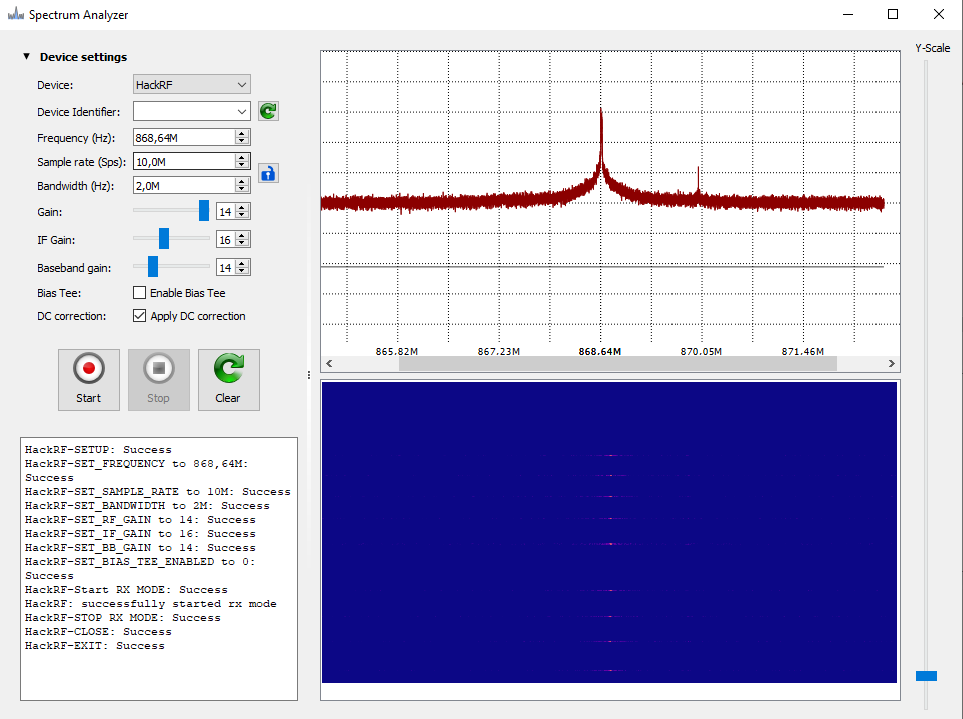
\includegraphics[width=0.9\textwidth]{images/6-pentesting/find-frequency.png}
    \caption{Finding the center frequency of the RF communication.}
    \label{fig:finding-center-freq}
\end{figure}

When the center frequency had been found, signals could be captured using URH's \textit{Record Signal} tool, see figure \ref{fig:rf-signal-capture}. This tool records raw audio signals captures from the HackRF. In the menu options, one has to select the correct frequency. After some trial and error, \texttt{868.638 MHz} was found to yield good captured signals. By placing the HackRF close to the devices, the SDR was able to capture clean signals without increasing the gain parameters. See figure \ref{fig:rf-lab-setup} for the physical set up. By zooming into the captured audio signals and seeing clear sinusoidal waves with a non-trivial pattern, one could verify that the capture was most likely done correctly. Figure \ref{fig:zoomed-in-signal} shows a good signal captured from the door sensor's temper alarm. This was done for all identified communication endpoints of the system.
\begin{figure}[!ht]
    \centering
    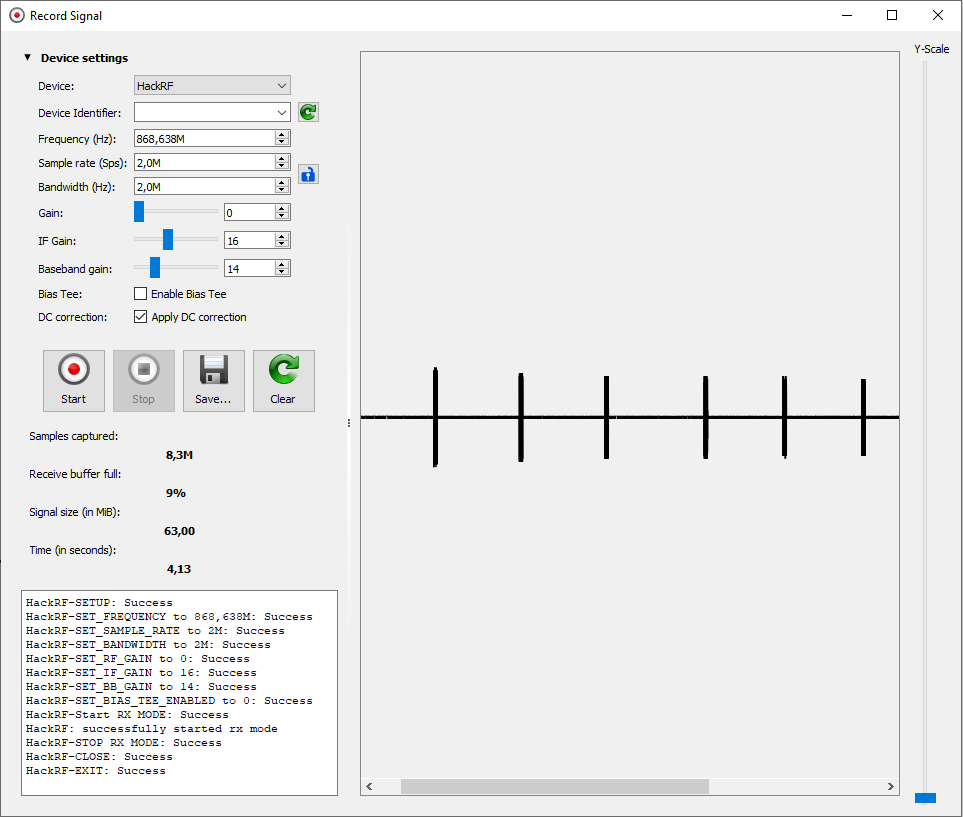
\includegraphics[width=0.9\textwidth]{images/6-pentesting/signal-capture.png}
    \caption{Capturing an RF signal using Universal Radio Hacker.}
    \label{fig:rf-signal-capture}
\end{figure}
\begin{figure}[!ht]
    \centering
    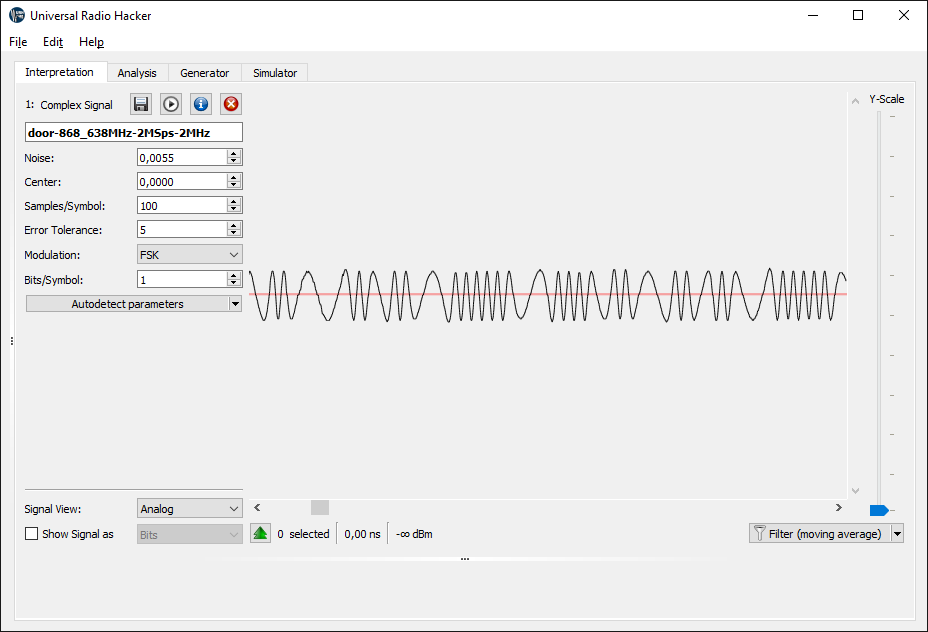
\includegraphics[width=0.9\textwidth]{images/6-pentesting/zoomed-in-signal.png}
    \caption{A cleanly captured RF signal, showing a clear sinusoidal pattern.}
    \label{fig:zoomed-in-signal}
\end{figure}

Lastly, once signals had been captured they could be replayed using URH's \textit{Send Signal} tool, see figure \ref{fig:uhr-replay-tool}. The tool lets you easily select and edit which parts of the captured signal to replay. Through a trial and error process, several combinations of packets were tested as a replay attack.
\begin{figure}[!ht]
    \centering
    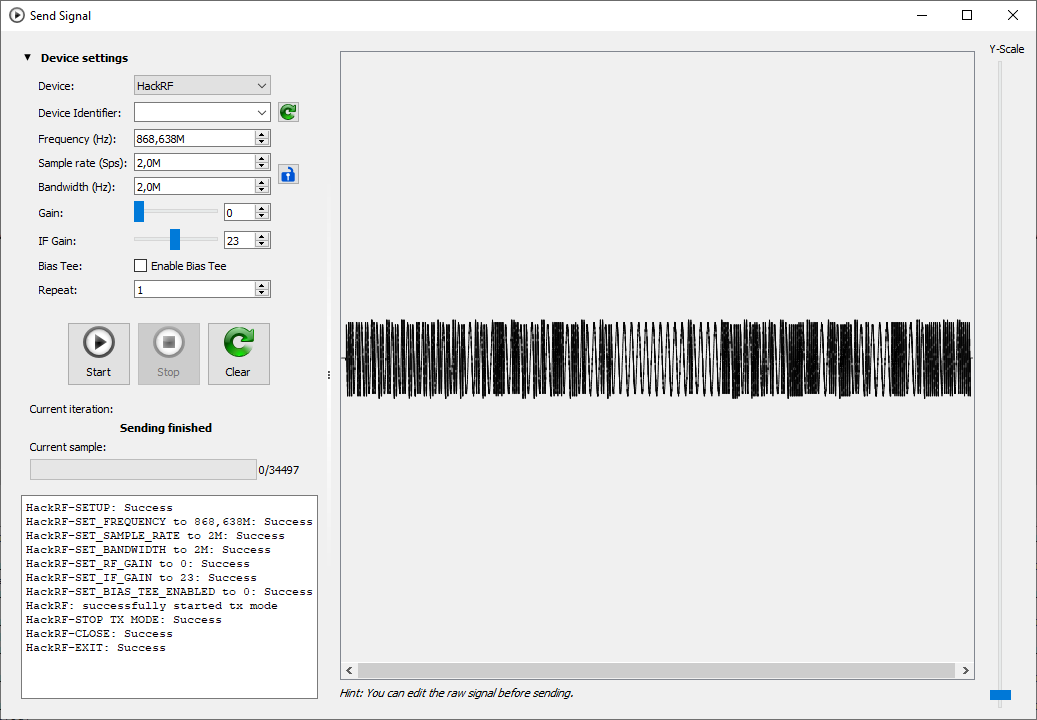
\includegraphics[width=0.9\textwidth]{images/6-pentesting/replay-signal.png}
    \caption{Performing a replay attack using Universal Radio Hacker.}
    \label{fig:uhr-replay-tool}
\end{figure}

\subsection{Results}
This test was successful and revealed \textit{critical} security flaws in the system. Every single tested endpoint of the RF communication were deemed vulnerable to replay attacks. The communication endpoints tested include the following:
\begin{itemize}
    \item Arming and disarming the alarm from the remote keypad.
    \item Triggering/resolving the tamper sensor of the door sensor.
    \item Triggering/resolving the tamper sensor of the camera.
    \item Triggering/resolving the tamper sensor of the main panel.
\end{itemize}
This has critical consequences for the security of the system. Capturing the RF signal of the user arming and disarming the alarm gives an attacker complete control of the arming state of the system. By simply replaying the signal, the main panel perceives this as a valid signal coming from the remote keypad.

\subsection{Discussion}
The system seems to have no protection against replay attacks what so ever. In fact, replaying the signals several \textit{weeks} later was still successful. However, replaying the signals against a different system of the same model was tested and it was unsuccessful. Presumably, some kind of ID of the device is sent making the packets invalid for another copy of the system. It clearly shows that the manufacturer, Climax Technology, either lacks the knowledge and competence to implement secure RF communication or have decided not to prioritize security at the RF layer. Either way this is a big mistake on their part. SDRs have become much more available and much cheaper in the last years. Attackers now have access to RF attacks which would have just a couple of years ago required very expensive and difficult to acquire hardware.

Furthermore, there are some factors that would make this attack easier for an attacker in practice. When trying this attack signals were first incorrectly recorded at \texttt{868.0 MHz} instead of the correct frequency at \texttt{868.64 MHz}, giving rise to a very spiky signal. Still the replay attack worked using this signal without issue. This indicates that perhaps the signal does not have to captured that cleanly and that a badly captured signal, say from a distance or outside of the house, could be used to perform a replay attack. Presumably, the system implements some kind of error correction and noise filtering to increase the range and reliability of the RF communication. Additionally, regarding the tamper sensor signals, six signals are sent after one and other, see figure \ref{fig:rf-signal-capture}. However, replaying only one of them still yields a successful replay attack. All of the six packets work individually. Presumably, the system repeats the same or similar signal several times for redundancy, in case one gets lost or corrupted in transit. This means, however, that an attacker only has to capture one of them to be able to perform a replay attack.

\section{Task 4: Insecure default credentials}
This section covers the topic of insecure default credentials. It does not include a \textit{pentest}, per se, but instead a list of all such credentials discovered in the system. These were discovered during the exploratory phase, and threat modeling phase of the project. Therefore, this section does not include a method part.

\subsubsection{Background}
Often default credentials are unavoidable. When first accessing the system, you need some way to do that without having authenticated yourself before. These credentials can, however, be more or less secure. A huge problem within cybersecurity is using insecure default credentials that can be easily guessed by a hacker. Additionally, often the user is never forced or even encouraged to change these credentials, leading to a potentially severe vulnerability. A common example is routers, which almost always feature an admin page to configure settings. Usually, all routers of the same model have the same default login credentials and often these are as simple as \texttt{admin:admin}. This is such a common issue that there are public databases of these passwords for each model \footnotelink{www.routerpasswords.com}{2021-0501}. Often the owner of the router is not even aware that this page exists or that they should change the password.

Famously, the MIRAI botnet relied on insecure default credentials to hack into hundreds of thousands of devices. It used just \texttt{62} different credentials \cite{understanding-mirai}. MIRAI is a worm malware, which targeted mostly IoT devices. It looked for devices with TCP port 23 or 2323 open, which are both often used by Telnet, and tried these credentials there. After gaining successful authentication against the device, these credentials and IP would be sent to a central server. Using this technique, over half a million devices were hacked and incorporated into the MIRAI botnet, which in turn was able to perform large scale DDOS attacks against websites. It was able to reach almost \texttt{1 TB/s} against a single target.

\subsubsection{Results}
The system can be armed and disarmed via the remote keypad (see section \ref{fig:hardware-components}) by entering a personal four-digit pin. By default, this is set to \texttt{1234}. You are never forced or even encouraged to enter a new code, overriding the easily-guessable default.

Additionally, when an alarm is triggered Securitas will send security personnel to inspect the site. If you accidentally triggered the alarm yourself Securitas has a phone number you can call to cancel the alarm. However, as a security mechanism, when doing this you have to correctly say a four-digit code (different from the previously discussed code). If you do not remember your code or say it incorrectly personnel will be sent to the site regardless. This code is by default the last four digits of \textit{your phone number}. Once again, you are never forced or even encouraged by the system to change this code.

No other bad default credentials were found. Importantly, the local admin panel (see section \ref{ch:system:software}) does not seem to use bad default credentials. Several hundred common default passwords were tried and none of them were successful (see section \ref{ch:pentesting:password}).

\subsubsection{Discussion}
Two insecure default credentials were discovered in the system. The first one, the arming pin defaulting to \texttt{1234}, is relatively severe. After triggering an alarm, you have a set time interval to disable it using your personal four-digit pin before the alarm is sent to the alarm center. An attacker could bet on the fact that this code has not been changed, and use it to turn off an alarm after breaking into the house. One could argue, however, that the probability of someone not changing this code is relatively low. The code arguably has an \textit{obvious} insecurity, leading to people perhaps feeling a greater need to change it. However, using a random code as the default would be substantially more secure.

The second code, used to call off an active alarm, is also a security issue. Your address and phone number can often easily be tied to one another and looked up using publicly available resources. An attacker obviously has the address if they are trying to get access to the house. Finding the phone number of the resident could be done in seconds using public websites for example. However, people can have multiple phone numbers and the house can of course have multiple residents.

Both identified insecure default credentials require the attacker to take quite a big risk to be able to exploit. An attacker would have to break into a house and only afterward bet on the fact that these had not been changed. One could then either turn off the alarm or try and call the alarm central before the owner does. All while the owner has been notified of an alarm breach via both email and the mobile app (see section \ref{ch:system:software}). While perhaps not critical vulnerabilities, they are nevertheless completely unnecessary. The system could easily give you a random code instead or force you to enter one upon first registering the system. Giving it an insecure default or tying it to publicly available information is not ideal and can be easily avoided.

